\begin{multicols}{3}
\byline{Интервю с  г-жа Софка Бубалова, заместник директор на гимназия 
„Гьоте”}{Вяра Тъпчева и Мария Ташева, X д клас}

Г-жо Бубалова, Вие сте дълги години преподавател и след това зам. Директор на 
гимназия Гьоте. Какво си спомняте от първите години на Вашата кариера?

-Ако това, че съм учител, може да се назове кариера, защото аз съм учител по 
призвание. За мен както и днес, така и през първите години беше и все още е 
удоволствие да работя в гимназията. За първите години си спомням, че бях много 
добре посрещната от колегите, цареше  една прекрасна атмосфера, едно пълно 
разбирателство между учителите и учениците. Затова си спомням с най-добро 
чувство за първите години в гимназията.

Можете ли да ни опишете как протича един ваш ден?

-О, много интензивно наистина. Защото освен преподавателската ми работа и 
влизането в часове по немски език, работата ми е свързана и с административна 
дейност като помощник директор.  Не в този чист смисъл администрация, ами 
по-скоро се състои в провеждане на много срещи, разговори, организиране на 
олимпиади, съставяне на комисии, провеждане на изпити и още много много други 
неща.

Кои бяха предизвикателствата пред вас през последните години?

-Бяха и все още са, бих казала. За мен най-голямото предизвикателство е, че 
времето е много динамично и нещата се променят наистина бързо. 
Предизвикателството пред мен е, че се стремя да бъда в крак с тази динамика и с 
промените в цялото общество, като същевременно се стремя да запазя ценностите в 
хората.Опитвам се да ги опазя доколкото мога, като под ценности разбирам- 
доброта, всеотдайност, уважение, разбирателство в отношения: учители- ученици, 
учители-родители, във всички тези страни, които участват в учебно възпитателния 
процес в гимназията.

\begin{window}[2,r, 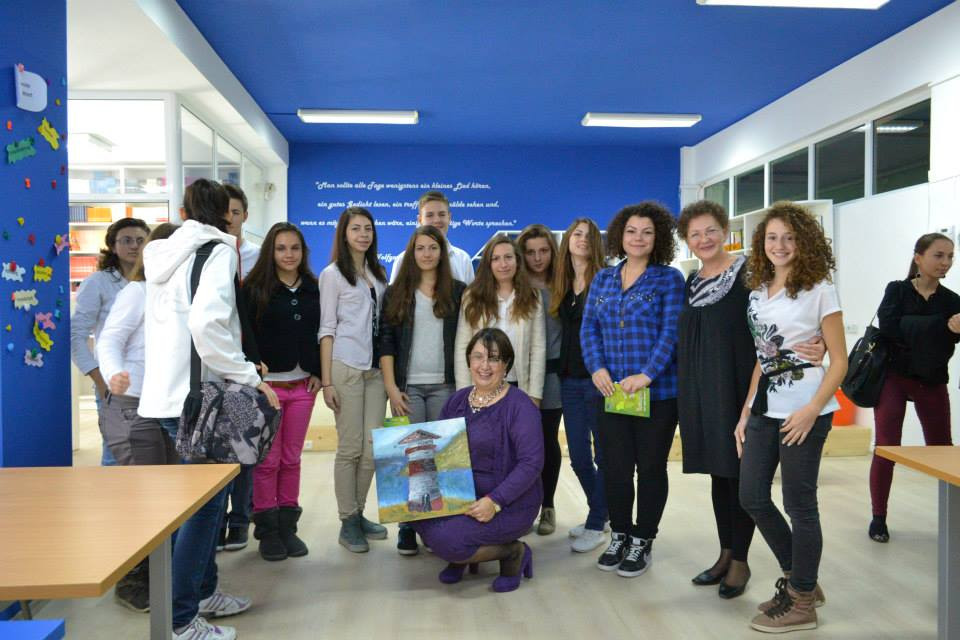
\includegraphics[width=4.4in]{./Bubalova/4.jpg},] \end{window}


Кое от ежедневието на гимназията Ви радва най-много и Ви кара най-искрено да се 
усмихнете?

-Бих казала, че най-много радост ми носи една искрена усмивка и тя би ме 
накарала и аз да се усмихна. Радвам се, когато всички ние, които сме в 
гимназията, я приемаме като своя, независимо дали като работно място или място 
за учене, и участваме в нейния живот, даваме всичките си сили в името на 
гимназията; когато усещам, че всички работим заедно.

Как бихте желали да изглежда бъдещето на гимназията? 

-Бих желала гимназията да запази традициите си; бих желала облика на гимназията 
,който  тя има като част от живота  в този нас прекрасен град-Бургас  да се 
запази такъв  и бих желала 100% от нашите ученици да завършат със сертификат 
„Езикова диплома”; бих желала нашите ученици да бъдат винаги най-добритеи на първите\\[8cm] 

\noindent местав олимпиади,състезания и тн.; бих желала....мога да изброявам още 
много неща.

Разкажете ни за едно от Вашите начинания – да ръководите клуб „Млад преводач”, 
начинание, което може би е първото по рода си в страната.

–Да така е, смея и аз да го твърдя. Идеята се  роди когато Eвропейската комисия 
обяви едно състезание “Млад преводач”  и ние участвахме в него. Това съвпадна с 
50-годишнината на гимназията и тогава се създаде клубът; срещна голям отклик в 
младите хора в  гимназията и мисля, че учениците разбраха също, че това е едно 
обогатяване, защото преводът е мост между културите  и човек трябва да познава и 
собствения си език и също така чуждия, за да успее да направи хубав превод.  
Мисля ,че постигнахме много неща, освен участията  в този конкурс на  
Европейската комисия, също и издадохме сборник  „Млад преводач” . Много често 
сме участвали в инициативи на „Гьоте институт” ,на община Бургас, когато имат 
нужда от млади преводачи за мероприятия в Морското казино. Проведохме среща с 
една от най-добрите преводачки в България- Марияна Хил. Много емоционална, много 
хубава среща и така работата на клуб „Млад преводач” продължава. В момента 
работим върху превода на интернет страницата на  гимназията и се надяваме до 
юбилейната седмица това също да стане факт,  да има интернет страница и на 
немски език.

Какво можете да ни разкажете за другата Ваша страст- театъра и ръководената от 
Вас театрална трупа на гимназията?

-Вие казахте страст, аз го наричам и привързаност. С много обич създадох 
театралната трупа през 2001-2002 г.Нашите театрални сезони съвпадат с учебните 
години,така и ги наричаме, а в момента тече сезон 2014-2015г. За мен театърът е 
част от живота, но театъра дава и възможност на младите хора да покажат на 
сцената онова,което се случва в ежедневието ни,да се превъплътят в много роли и 
тъй като участват с всичките си сетива, с гласа си и с мимика и жест, мисля, че 
тетърът дава много на младите хора, а да играем на сцената на драматичен театър 
„Адриана Будевска”, това си е истинско предизвикателство,но аз мисля ,че нашите 
млади театрали се справят с него. Факт е, че вече имаме четирима наши 
ученици,които са или актьори  или в момента студенти в  НАТФИЗ , започвам с 
Илияна Куджабашева, Екатерина Георгиева, Никола Парашкевов, който вече е и 
актьор в „Адриана Будевска”, а в момента студент е нашият възпитаник  Александър 
Валериев. Не си преписвам заслугите на мен, това са заслуги на младите хора, но 
мисля, надявам се тази театрална трупа да продължи своята дейност и през  
годините.

Какво е Вашето послание към колегите Ви и учениците на гимназията по случай 55 
годишния юбилей? 

–Много неща могат да се пожелаят. Аз ще бъда съвсем кратка.  Да не губят 
дръзновението и любознателността си, всеотдайността си и през следващите 
десетски лета. Да бъдат винаги на висотата на  мечтите си, за да се множат 
успехите на гимназията, за да могат да казват  с гордост, както и до сега: „Аз 
съм от немската в Бургас”, защото и аз съм от немската в Бургас.

\closearticle
\end{multicols}